\section{Improper Integrals}
So far, we have only examined integrals of continuous, or at
least bounded functions. Let's see how to deal with a more general
collection of functions!

In particular, we will examine two types:
\begin{enumerate}[label=(\arabic*)]
    \item Continuous functions over infinite intervals
    \item Functions with infinite discontinuities
\end{enumerate}

In particular:
\begin{itemize}
    \item Type I\@: Infinite Intervals. Integrals of the form
          $ \displaystyle \int_{-\infty}^{a} f(x)\, d{x},\,
              \int_{a}^{\infty} f(x)\, d{x},\text{ or }
              \int_{-\infty}^{\infty} f(x)\, d{x} $.
    \item Type II\@: Infinite Discontinuity. For example,
          $ \displaystyle \int_{-1}^{1} \frac{1}{x} \, d{x} $
          as there is an issue at $ x=0 $.
\end{itemize}

In all cases, the idea is to replace the problematic point with a
letter and take a limit.

Let's see them in more detail now!

\subsection*{Type I}
We replace the infinite endpoint with a letter and take a limit
\begin{itemize}
    \item $ \displaystyle \int_{-\infty}^{a} f(x)\, d{x} =\lim\limits_{{b} \to {-\infty}}
              \int_{b}^{a} f(x)\, d{x} $
    \item $ \displaystyle \int_{a}^{\infty} f(x)\, d{x} =\lim\limits_{{b} \to {\infty}}
              \int_{a}^{b} f(x)\, d{x} $
    \item $ \displaystyle  \int_{-\infty}^{\infty} f(x)\, d{x}=
              \lim\limits_{{b_1} \to {-\infty}} \int_{b_1}^{0} f(x)\, d{x}+
              \lim\limits_{{b_2} \to {\infty}} \int_{0}^{b_2} f(x)\, d{x} $
\end{itemize}
\begin{Remark}{}{}
    Don't use
    $ \displaystyle \int_{-\infty}^{\infty} f(x)\, d{x}=\lim\limits_{{b} \to {\infty}}
        \int_{-b}^{b} f(x)\, d{x} $.
    This is called the ``Cauchy Principal Value'' and it is something else!
\end{Remark}


We say that the integral \textbf{converges} if all the limits exist
(and are finite). The integral \textbf{diverges} if even one limit does
not exist (or is $ \pm\infty $).

\begin{Example}{Type I Integrals}{}
    Evaluate the following or show they diverge.
    \begin{enumerate}[label=(\roman*)]
        \item $ \displaystyle \int_{2}^{\infty} \frac{1}{x^2} \, d{x} $

              \textbf{Solution.}
              \[
                  \int_{2}^{\infty} \frac{1}{x^2} \, d{x}
                  =\lim\limits_{{b} \to {\infty}} \int_{2}^{b} \frac{1}{x^2} \, d{x}       \\
                  = \lim\limits_{{b} \to {\infty}} \left[-\frac{1}{x}  \right]_{2}^b       \\
                  =\lim\limits_{{b} \to {\infty}} \left( -\frac{1}{b} +\frac{1}{2} \right) \\
                  =\frac{1}{2}
              \]
              Thus, the integral converges.
        \item $ \displaystyle \int_{-\infty}^{\infty} \sin(x)\, d{x} $

              \textbf{Solution.}
              \[
                  \int_{-\infty}^{\infty} \sin(x)\, d{x}
                  =\lim\limits_{{b_1} \to {-\infty}} \int_{b_1}^{0} \sin(x)\, d{x}
                  +\lim\limits_{{b_2} \to {\infty}} \int_{0}^{b_2} \sin(x)\, d{x}
              \]
              Let's evaluate the first one:
              \[ \lim\limits_{{b_1} \to {-\infty}}\int_{b_1}^{0} \sin(x)\, d{x}
                  = \lim\limits_{{b_1} \to {-\infty}}\bigl[-\cos(x) \bigr]_{b_1}^0
                  =\lim\limits_{{b_1} \to {-\infty}} \left[-\cos(0)+\cos(b_1)\right] \]
              which does not exist. Therefore, this integral
              diverges, there is no need to check the second limit!
        \item $ \displaystyle \int_{0}^{\infty} \frac{1}{1+x^2}\, d{x} $

              \textbf{Solution.}\begin{align*}
                  \int_{0}^{\infty} \frac{1}{1+x^2}\, d{x}
                   & =\lim\limits_{{b} \to {\infty}} \int_{0}^{b} \frac{1}{1+x^2} \, d{x} \\
                   & = \lim\limits_{{b} \to {\infty}} \bigl[\arctan(x) \bigr]_{0}^b       \\
                   & =\lim\limits_{{b} \to {\infty}} \left[\arctan(b)-\arctan(0) \right]  \\
                   & =\frac{\pi}{2} -0                                                    \\
                   & =\frac{\pi}{2}
              \end{align*}
              Thus, the integral converges.
    \end{enumerate}
\end{Example}
Question: For which $ p\in\mathbb{R} $ does $ \displaystyle \int_{1}^{\infty} \frac{1}{x^p} \, d{x} $
converge?

Let's find out!

\begin{Proof}{\ref{thm:p-int}}{}
    \underline{Case 1}: $ p>1 $.
    \[
        \lim\limits_{{b} \to {\infty}} \int_{1}^{b} x^{-p}\, d{x}
        = \lim\limits_{{b} \to {\infty}} \left[\frac{x^{-p+1}}{-p+1}  \right]_{1}^b
        =\lim\limits_{{b} \to {\infty}} \left( \frac{b^{-p+1}}{-p+1}-
        \frac{1^{-p+1}}{-p+1}  \right)
        =\frac{1}{p-1}
    \]
    since $ -p+1<0 $, so $ b^{-p+1}\to 0 $. So, the integral converges if $ p>1 $.

    \underline{Case 2}: $ p<1 $. The calculation is the same as Case 1, until:
    \[ \lim\limits_{{b} \to {\infty}} \left( \frac{b^{-p+1}}{-p+1} -\frac{1}{-p+1}\right) =\infty  \]
    since $ -p+1>0 $, so $ b^{-p+1}\to\infty $. So, the integral diverges if $ p<1 $.

    \underline{Case 3}: $ p=1 $.
    \[
        \lim\limits_{{b} \to {\infty}} \int_{1}^{b} \frac{1}{x} \, d{x}
        =\lim\limits_{{b} \to {\infty}} \bigl[\ln\abs{x}\bigr]_{1}^b
        =\lim\limits_{{b} \to {\infty}} \left( \ln\abs{b}-\ln\abs{1} \right)
        =\infty
    \]
    So, the integral diverges if $ p=1 $.
\end{Proof}

Therefore, we have proven:

\begin{Theorem}{$p$-Integrals}{p-int}
    The improper integral
    $ \displaystyle \int_{1}^{\infty} \frac{1}{x^p} \, d{x}  $
    converges if and only if $ p>1 $.
    If $ p>1 $,
    $ \displaystyle \int_{1}^{\infty} \frac{1}{x^p} \, d{x} =\frac{1}{p-1} $.
\end{Theorem}

Next, let's examine some properties of Type I improper integrals.

\begin{Theorem}{Properties of Type I Improper Integrals}{}
    Suppose $ \displaystyle \int_{a}^{\infty} f(x)\, d{x}  $ and
    $ \displaystyle \int_{a}^{\infty} g(x)\, d{x}  $
    both converge.
    \begin{enumerate}[label=(\arabic*)]
        \item $ \displaystyle \int_{a}^{\infty} cf(x)\, d{x} $
              converges for any $ c\in\mathbb{R} $, and
              \[ \int_{a}^{\infty} cf(x)\, d{x} =c \int_{a}^{\infty} f(x)\, d{x} \]
        \item $ \displaystyle \int_{a}^{\infty} f(x)+g(x)\, d{x} $
              converges, and
              \[ \int_{a}^{\infty} f(x)+g(x)\, d{x}=
                  \int_{a}^{\infty} f(x)\, d{x} +\int_{a}^{\infty} g(x)\, d{x} \]
        \item If $ f(x)\leqslant g(x) $ for all $ x\geqslant a $, then
              \[ \int_{a}^{\infty} f(x)\, d{x} \leqslant \int_{a}^{\infty} g(x)\, d{x} \]
        \item If $ a<c<\infty $, then $ \int_{c}^{\infty} f(x)\, d{x} $ converges, and
              \[ \int_{a}^{\infty} f(x)\, d{x}=
                  \int_{a}^{c} f(x)\, d{x} +\int_{c}^{\infty} f(x)\, d{x} \]
    \end{enumerate}
\end{Theorem}
Evaluating integrals in general is hard, and determining if an improper integral converges
may be even harder! However, we do have a way of comparing a difficult
integral to a simpler one (for example, a $ p $-Integral!).

\subsubsection{The Comparison Theorem (For Type I)}
\begin{Theorem}{Comparison Test for Type I Improper Integrals}{}
    Assume $ 0\leqslant g(x)\leqslant f(x) $ for all $ x\geqslant a $
    and that both $ f $ and $ g $ are continuous on $ \interval[open right]{a}{\infty} $.
    \begin{enumerate}[label=(\arabic*)]
        \item If $ \displaystyle \int_a^{\infty}f(x)\, d{x} $ converges, then so does
              $ \displaystyle \int_a^{\infty}g(x)\, d{x} $.
        \item If $ \displaystyle \int_a^{\infty}f(x)\, d{x} $ diverges, then so does
              $ \displaystyle \int_a^{\infty}g(x)\, d{x} $.
    \end{enumerate}
\end{Theorem}
\begin{Example}{}{}
    Determine if $ \displaystyle \int_0^\infty e^{-x^2}\, d{x} $ converges or diverges.

    \textbf{Solution.} Note for $ x>1 $,
    $ 0\leqslant e^{-x^2} <e^{-x} $, by comparison since
    $ \displaystyle \int_{0}^{\infty} e^{-x^2}\, d{x} $ converges, so does
    $ \displaystyle \int_{0}^{\infty} e^{-x^2}\, d{x} $.
\end{Example}
\begin{Remark}{}{}
    It doesn't matter that the inequality doesn't hold for $ 0\leqslant x<1 $,
    since $ \int_{0}^{1}e^{-x^2} \, d{x} $ is not improper and so converges.
\end{Remark}

\begin{Example}{}{}
    Determine of the following integrals converge or diverge.
    \begin{enumerate}[label=(\roman*)]
        \item $ \displaystyle \int_{1}^{\infty} \frac{x}{(x^2+2)^2}\, d{x} $.

              \textbf{Solution.} Note that
              $ \displaystyle  0\leqslant \frac{x}{(x^2+2)^2}\leqslant \frac{x}{x^4}=\frac{1}{x^3} $,
              for $ x\geqslant 1 $.

              Since $ \displaystyle \int_{1}^{\infty} \frac{1}{x^3} \, d{x}  $
              converges ($ p $-integral), so does $ \displaystyle \int_{1}^{\infty} \frac{x}{(x^2+2)^2} \, d{x} $,
              by comparison.
        \item $ \displaystyle \int_{1}^{\infty} \frac{2x^2}{x^3-x+1} \, d{x}  $.

              \textbf{Solution.} Note that
              $ \displaystyle \frac{2x^2}{x^3-x+1} \geqslant \frac{2x^2}{x^3+1} \geqslant \frac{2x^2}{x^3+x^3}=
                  \frac{2}{2x} =\frac{1}{x}\geqslant 0 $,
              for $ x\geqslant 1 $.

              Since $ \displaystyle \int_{1}^{\infty} \frac{1}{x} \, d{x}  $
              diverges ($ p $-integral), so does $ \displaystyle \int_{1}^{\infty} \frac{2x}{x^3-x+1} \, d{x} $,
              by comparison.
        \item $ \displaystyle \int_{1}^{\infty} \frac{1+e^{-x}}{x} \, d{x} $.

              \textbf{Solution.} Note that
              $ \displaystyle \frac{1+e^{-x}}{x} \geqslant \frac{1}{x} \geqslant 0 $,
              for $ x\geqslant 1 $.

              Since $ \displaystyle \int_{1}^{\infty} \frac{1}{x} \, d{x}  $ diverges,
              so does $ \displaystyle \int_{1}^{\infty} \frac{1+e^{-x}}{x} \, d{x}  $, by comparison.
        \item $ \displaystyle \int_{0}^{\infty} \frac{e^x}{e^{2x}+3} \, d{x}  $.

              \textbf{Solution.} Note that
              $ \displaystyle  0\leqslant \frac{e^{x}}{e^{2x}+3} \leqslant \frac{e^{x}}{e^{2x}} =e^{-x} $,
              for $ x\geqslant 0 $.

              Since $ \displaystyle \int_{0}^{\infty} e^{-x}\, d{x}  $ converges,
              so does $ \displaystyle \int_{0}^{\infty} \frac{e^{x}}{e^{2x}+3} \, d{x}  $, by comparison.
    \end{enumerate}
\end{Example}

The comparison theorem is fantastic, but it only works on non-negative functions. How
can we deal with negative functions?

We can use absolute values!

\begin{Definition}{Absolute convergence}{}
    Let $ f $ be integrable on $ \interval[open right]{a}{b} $ for all $ b\geqslant a $.
    We say that the improper integral $ \displaystyle \int_{a}^{\infty} f(x)\, d{x} $
    \textbf{converges absolutely} if
    $ \displaystyle \int_{a}^{\infty} \abs{f(x)}\, d{x} $
    converges.
\end{Definition}

\begin{Theorem}{Absolute Convergence Theorem (ACT)}{act_int}
    Let $ f $ be integrable on $ \interval{a}{b} $ for all $ b\geqslant a $.
    Then $ \abs{f} $ is also integrable on $ \interval{a}{b} $ for all $ b\geqslant a $.
    Moreover, if we assume that
    $ \displaystyle \int_{a}^{\infty} \abs{f(x)}\, d{x} $
    converges, then so does
    $ \displaystyle  \int_{a}^{\infty} f(x)\, d{x} $.

    In particular, if $ \abs{f(x)}\leqslant g(x) $ for all $ x\geqslant a $,
    both $ f $ and $ g $ are integrable on $ \interval{a}{b} $ for all $ b\geqslant a $,
    and if $ \displaystyle \int_{a}^{\infty} g(x)\, d{x}  $ converges, then so does
    $ \displaystyle \int_{a}^{\infty} f(x)\, d{x} $.
\end{Theorem}

\begin{Proof}{\ref{thm:act_int}}{}
    Suppose $ \int_{a}^{\infty} \abs{f(x)}\, d{x} $ converges. Then so does
    \[ \int_{a}^{\infty} 2\abs{f(x)}\, d{x}. \]
    Note that
    \[ 0\leqslant f(x)+\abs{f(x)}\leqslant 2\abs{f(x)}, \]
    so by comparison,
    \[ \int_{a}^{\infty} f(x)+\abs{f(x)}\, d{x} \]
    converges. But
    \[ \int_{a}^{\infty} f(x)\, d{x} =\int_{a}^{\infty} f(x)+\abs{f(x)}\, d{x} -
        \int_{a}^{\infty} \abs{f(x)}\, d{x}  \]
    converges, since both components do.
\end{Proof}

\begin{Example}{}{}
    Determine if $ \displaystyle \int_{1}^{\infty} \frac{\sin(x)}{x^2+1} \, d{x} $
    converges or diverges.

    \textbf{Solution.}
    We can't use comparison directly since $ \sin(x)<0 $ sometimes. But,
    \[ \displaystyle  0\leqslant \abs*{\frac{\sin(x)}{x^2+1} }\leqslant \frac{1}{x^2+1}
        \leqslant \frac{1}{x^2} \]
    for $ x\geqslant 1 $, and $ \displaystyle \int_{1}^{\infty} \frac{1}{x^2} \, d{x}  $ converges. So by
    ACT, $ \displaystyle \int_{1}^{\infty} \frac{\sin(x)}{1+x^2} \, d{x}  $ converges.
\end{Example}

Now, let's switch to Type II improper integrals. We will see how to deal with them, but we won't
go as deeply into them.

\subsection*{Type II}
Consider $ \displaystyle \int_{a}^{b} f(x)\, d{x}  $.
\begin{itemize}
    \item If $ f $ has an infinite discontinuity at $ x=a $, then we use
          \[ \int_{a}^{b} f(x)\, d{x} =\lim\limits_{{t} \to {a^+}} \int_{t}^{b} f(x)\, d{x} \]
    \item If $ f $ has an infinite discontinuity at $ x=b $, then we use
          \[ \int_{a}^{b} f(x)\, d{x} =\lim\limits_{{t} \to {b^-}} \int_{t}^{b} f(x)\, d{x} \]
    \item If $ f $ is not continuous at $ c $, $ a<c<b $, then we write
          \[  \int_{a}^{b} f(x)\, d{x} =\int_{a}^{c} f(x)\, d{x} +\int_{c}^{b} f(x)\, d{x} \]
          and use the limits as the previous cases.
\end{itemize}
Again, if all limit(s) exist, then we say the integral \textbf{converges}. If even one
limit does not exist, then the integral \textbf{diverges}.

\begin{Example}{}{}
    Determine of the following integrals converge or diverge.
    \begin{enumerate}[label=(\roman*)]
        \item $ \displaystyle \int_{0}^{1} \frac{1}{\sqrt{1-x}} \, d{x} $.

              \textbf{Solution.} There is a problem at $ x=1 $. So,
              \[ \int_{0}^{1} \frac{1}{\sqrt{1-x}} \, d{x}
                  =\lim\limits_{{t} \to {1^-}} \int_{0}^{t} \frac{1}{\sqrt{1-x}} \, d{x}
                  =\lim\limits_{{t} \to {1^-}}\bigl[-2\sqrt{1-x}\bigr]_0^t
                  =\lim\limits_{{t} \to {1^-}}[-2\sqrt{1-t}+2\sqrt{1}]
                  =2
              \]
              Thus, the integral converges.
        \item $ \displaystyle \int_{2}^{3} \frac{x}{(x^2-4)^2}\, d{x}  $

              \textbf{Solution.} There is a problem at $ x=2 $,
              but let's make a substitution first! Let $ u=x^2-4 $, so $ du=2x\,dx $. If $ x=2 $,
              $ u=0 $, and if $ x=3 $, $ u=5 $. So,
              \[ \int_{2}^{3} \frac{x}{(x^2-4)^2}\, d{x}
                  =\int_{0}^{5} \frac{x}{u^2} \frac{1}{2x} \, d{u}
                  =\lim\limits_{{t} \to {0^+}} \frac{1}{2} \int_{t}^{5} \frac{1}{u^2}\, d{u}
                  =\lim\limits_{{t} \to {0^+}}\left[-\frac{1}{2u} \right]_t^5
                  =\lim\limits_{{t} \to {0^+}}\left[ -\frac{1}{10} +\frac{1}{2t} \right]
                  =\infty
              \]
              Thus, the integral diverges.
        \item $ \displaystyle \int_{0}^{3} \frac{1}{(x-2)^{\sfrac{1}{3} }}\, d{x}  $.

              \textbf{Solution.} There is a problem at $ x=2 $.
              \begin{align*}
                  \int_{0}^{3} \frac{1}{(x-2)^{\sfrac{1}{3} }}\, d{x}
                   & =\int_{0}^{2} \frac{1}{(x-2)^{\sfrac{1}{3}}} \, d{x}+\int_{2}^{3} \frac{1}{(x-2)^{\sfrac{1}{3} }} \, d{x} \\
                   & =\lim\limits_{{t_1} \to {2^-}} \int_{0}^{t_1} \frac{1}{(x-2)^{\sfrac{1}{3}}}  \, d{x} +
                  \lim\limits_{{t_2} \to {2^+}} \int_{t_2}^{3} \frac{1}{(x-2)^{\sfrac{1}{3}}} \, d{x}                          \\
                   & =\lim\limits_{{t_1} \to {2^-}} \left[ \frac{3}{2}(x-2)^{\sfrac{2}{3}}\right]_0^{t_1}+
                  \lim\limits_{{t_2} \to {2^+}}\left[ \frac{3}{2}(x-2)^{\sfrac{2}{3}}\right]_{t_2}^{3}                         \\
                   & =\lim\limits_{{t_1} \to {2^-}} \frac{3}{2} \left[ (t_1-2)^{\sfrac{2}{3}} -(0-2)^{\sfrac{2}{3}}\right]
                  +\lim\limits_{{t_2} \to {2^+}} \frac{3}{2} \left[ (3-2)^{\sfrac{2}{3}}-(t_2-2)^{\sfrac{2}{3}} \right]        \\
                   & =-\frac{3}{2} (-2)^{\sfrac{2}{3}}+\frac{3}{2}
              \end{align*}
              Thus, the integral converges.
    \end{enumerate}
\end{Example}

\begin{Exercise}{}{}
    Show $ \displaystyle \int_{0}^{1} \frac{1}{x^p} \, d{x}  $ converges if and only if $ p<1 $.
\end{Exercise}

\chapter{Applications of Integration}
\section{Area Between Curves}
Suppose we want to calculate the area of the region \emph{between} $ f $ and $ g $.

\begin{figure}[H]
    \centering
    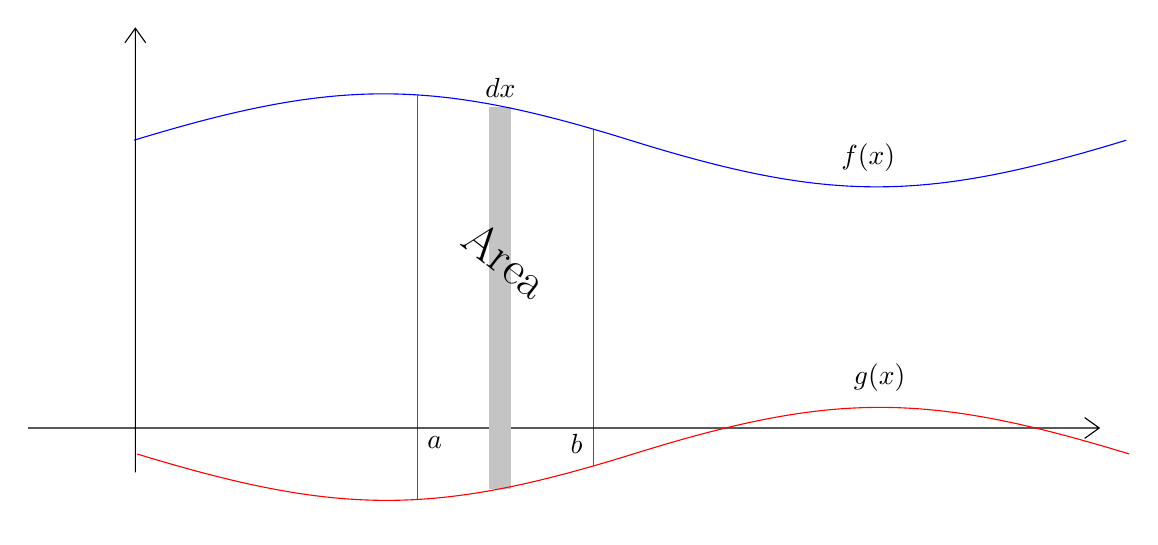
\begin{tikzpicture}[x=0.75pt,y=0.75pt,yscale=-1,xscale=1]
        %Straight Lines [id:da28604046841758335] 
        \draw [color={rgb, 255:red, 65; green, 117; blue, 5 }  ,draw opacity=1 ] (190,32) -- (190,227) ;
        %Straight Lines [id:da9682060697644969] 
        \draw [color={rgb, 255:red, 65; green, 117; blue, 5 }  ,draw opacity=1 ] (275,48.8) -- (275,211) ;
        %Shape: Axis 2D [id:dp044696932049605675] 
        \draw  (2.5,192.6) -- (518.5,192.6)(54.1,0) -- (54.1,214) (511.5,187.6) -- (518.5,192.6) -- (511.5,197.6) (49.1,7) -- (54.1,0) -- (59.1,7)  ;
        %Shape: Rectangle [id:dp19922766124111613] 
        \draw  [color={rgb, 255:red, 196; green, 196; blue, 196 }  ,draw opacity=1 ][fill={rgb, 255:red, 196; green, 196; blue, 196 }  ,fill opacity=1 ]
        (235,38) -- (235,221.87) -- (225,221.87) -- (225,38) -- cycle ;
        %Shape: Sine Wave Form [id:dp22033114506939577] 
        \draw  [color={rgb, 255:red, 0; green, 0; blue, 255 }  ,draw opacity=1 ] (53.5,53.95) .. controls (150.75,24.25) and (196.61,24.09) .. (292.47,53.95) .. controls (388.39,83.82) and (433.34,84) .. (531.5,53.95) ;
        %Shape: Sine Wave Form [id:dp021759591227149766] 
        \draw  [color={rgb, 255:red, 255; green, 0; blue, 0 }  ,draw opacity=1 ] (55,205.14) .. controls (152.25,234.84) and (198.11,235) .. (293.97,205.14) .. controls (389.89,175.28) and (434.84,175.09) .. (533,205.14) ;

        % Text Node
        \draw (193.5,195.4) node [anchor=north west][inner sep=0.75pt]    {$a$};
        % Text Node
        \draw (262.5,194.4) node [anchor=north west][inner sep=0.75pt]    {$b$};
        % Text Node
        \draw (393,54.4) node [anchor=north west][inner sep=0.75pt]    {$f(x)$};
        % Text Node
        \draw (399,160.4) node [anchor=north west][inner sep=0.75pt]    {$g(x)$};
        % Text Node
        \draw (230,34.6) node [anchor=south] [inner sep=0.75pt]    {$dx$};
        % Text Node
        \draw (219.85,90) node [anchor=north west][inner sep=0.75pt]  [font=\LARGE,rotate=-38.03] [align=left] {Area};
    \end{tikzpicture}
\end{figure}


This is the area under $ f $ \emph{minus} the area ``under'' (between $ g $ and the
$ x $-axis) $ g $.

Using the same ideas as before, we divide the region into infinitely many infinitely thin
rectangles (each with width $ \odif{x}\approx \Delta x $) and integrate!

Therefore, if $ f(x)\ge g(x) $ for all $ x\in[a,b] $, then the area bounded by
$ f(x) $ and $ g(x) $ from $ x=a $ to $ x=b $ is
\[ \int_{a}^{b} f(x)-g(x)\odif{x}. \]

\begin{Example}{}{}
    Find the area between $ f(x)=x^2 $ and $ g(x)=x $ from $ x=1 $ to $ x=3 $.

    \begin{center}
        \begin{tikzpicture}
            \begin{axis}[ylabel = $y$, xlabel = $x$, x post scale=1.4]
                \addplot[blue, domain=0:3.2, name path=F] {x^2} node [pos = 0.9, above left] {$y=x^2$};
                \addplot[red, domain=0:3.2, name path=G] {x} node [pos = 0.7, below right] {$y=x$};
                \draw[-] (1,9) -- (1,0) node[below] {$x=1$};
                \draw[-] (3,9) -- (3,0) node[below] {$x=3$};
                \addplot[fill=red!10] fill between [of=F and G, soft clip={domain=1:3}];
                \node[below] at (2.5,4.5) {Area};
            \end{axis}
        \end{tikzpicture}
    \end{center}

    \textbf{Solution}. Note that $ x^2\ge x $ for $ x\in[1,3] $, so we get
    \[ \text{Area}
        =\int_{1}^{3}x^2-x\odif{x}=\frac{14}{3}. \]
\end{Example}

\begin{Remark}{}{}
    You should always get a positive answer! If your answer is negative you should go check
    your work!

    Note that the ``upper'' curve may change over the interval.
\end{Remark}

\underline{Actual Formula}: Area between $ f $ and $ g $ from $ x=a $ to $ x=b $ is
\[ \int_{a}^{b} \abs{f(x)-g(x)}\odif{x}.  \]

So, we should split up the interval $ \interval{a}{b} $ to eliminate
the absolute value.

Remember, $ \displaystyle \int_{a}^{b} \text{``upper''}-\text{``lower''}\odif{x} $.

\begin{Example}{}{}
    Find the area enclosed by $ f(x)=1-x^2 $ and $ g(x)=x^2 $.

    \begin{center}
        \begin{tikzpicture}
            \begin{axis}[ylabel = $y$, xlabel = $x$]
                \addplot[blue, domain=-1.25:1.25, name path=F] {1-x^2} node [pos = 0.5, above] {$y=1-x^2$};
                \addplot[red, domain=-1.25:1.25, name path=G] {x^2} node [pos = 0.5, below] {$y=x^2$};
                \draw[-] ($ ({1/sqrt(2)}, 1) $) -- ($ ({1/sqrt(2)}, 0) $) node[below] {$x=\frac{1}{\sqrt{2}}$};
                \draw[-] ($ ({-1/sqrt(2)}, 1) $) -- ($ ({-1/sqrt(2)}, 0) $) node[below] {$x=-\frac{1}{\sqrt{2}}$};
                \addplot[fill=red!10] fill between [of=F and G, soft clip={domain=-0.7071:0.7071}];
                \node[below] at (0,0.5) {Area};
            \end{axis}
        \end{tikzpicture}
    \end{center}

    \textbf{Solution}. First, we need to find the intersection points:
    $ \displaystyle 1-x^2=x^2\iff 1=2x^2\iff x=\pm \frac{1}{\sqrt{2}} $.

    Note that $ 1-x^2\ge x^2 $ for $ \displaystyle  x\in\biggl[-\frac{1}{\sqrt{2}},\frac{1}{\sqrt{2}}\biggr] $,
    so we get
    \[ \text{Area}=\int_{-1/\sqrt{2}}^{1/\sqrt{2}}(1-x^2)-(x^2)\odif{x}=\frac{2\sqrt{2}}{3}. \]
\end{Example}

\begin{Example}{\emph{This example number reminds me of $ \pi $, but not quite $ \pi $.}}{}
    Find the area between $ f(x)=\sin(x) $ and $ g(x)=\cos(x) $ from $ x=0 $ to $ x=\pi $.


    \begin{center}
        \begin{tikzpicture}
            \begin{axis}[ylabel = $y$, xlabel = $x$, x post scale=1.4,
                    xtick={0,1.57,3.14},
                    xticklabels={$0$, $\frac{\pi}{2}$,$\pi$}]
                \addplot[blue, domain=0:pi, name path=F] {sin(deg(x))} node [pos = 0.7, above right] {$y=\sin x$};
                \addplot[red, domain=0:pi, name path=G] {cos(deg(x))} node [pos = 0.5, below left] {$y=\cos x$};
                \addplot[fill=red!10] fill between [of=F and G, soft clip={domain=0:pi}];
                \node[below] at (0.25,0.75) {$A_1$};
                \node[below] at (2,0.5) {$A_2$};
                \draw[-] (0,1) -- (0,-1) node[below] {$x=0$};
                \draw[-] (pi,1) -- (pi,-1) node[below] {$x=\pi$};
                \draw[-] (pi/4,1) -- (pi/4,-1) node[below] {$x=\pi/4$};
            \end{axis}
        \end{tikzpicture}
    \end{center}

    \textbf{Solution}. Note that
    $ \cos x\ge \sin x $ for $ x\in[0,\pi/4] $ and
    $ \sin x\ge \cos x $ for $ x\in[\pi/4,\pi] $, so we get
    \[ \text{Area}
        =A_1+A_2\\
        =\int_{0}^{\pi/4}\cos x-\sin x\odif{x}+\int_{\pi/4}^{\pi}\sin x-\cos x\odif{x}
        =2\sqrt{2}. \]

\end{Example}

We can use the same ideas to compute areas when $ x $ is a function of $ y $, except we use
\[ \text{``outer''}-\text{``inner''}\text{ or }\text{``right''}-\text{``left''}\]

\begin{Example}{}{}
    Find the area between $ x=y^2+1 $ and $ y=x $ from $ y=0 $ to $ y=2 $.

    \begin{center}
        \begin{tikzpicture}
            \begin{axis}[ylabel = $y$, xlabel = $x$, x post scale=1.4]
                \addplot[blue, domain=1:5.5, name path=F] {sqrt(x-1)} node [pos = 0.8, below right] {$x=y^2+1$};
                \addplot[blue, domain=1:5.5] {-sqrt(x-1)};
                \addplot[red, domain=0:2, name path=G] {x} node [pos = 0.5, above left] {$y=x$};
                \addplot[black, domain=0:5.5] {0} node [pos = 0, below] {$y=0$};
                \addplot[black, domain=0:5.5] {2} node [pos = 0, above] {$y=2$};
                \addplot[fill=red!10] fill between [of=F and G, soft clip={domain=0:5}];
                \node[below] at (2.5,1.75) {Area};
            \end{axis}
        \end{tikzpicture}
    \end{center}

    \textbf{Solution 1}. Note that $ y^2+1\ge y $ for $ y\in[0,2] $, so
    \[\text{Area}
        =\int_{0}^{2}(y^2+1)-(y)\odif{y}
        =\frac{8}{3}. \]
    \textbf{Solution 2}. If we wanted to work with functions of $ x $ instead,
    we could equivalently compute
    \[ \text{Area}=\int_{0}^{1}x\odif{x}+\int_{1}^{2}x-\sqrt{x-1}\odif{x}+\int_{2}^{5}2-\sqrt{x-1}\odif{x}=\frac{8}{3}. \]
\end{Example}
